\begin{figure}[t] 
    \setlength{\abovecaptionskip}{-0cm}
    \setlength{\belowcaptionskip}{-0.5cm}
	\subfigtopskip=2pt 
	\subfigbottomskip=2pt 
	\subfigcapskip=-5pt
	\subfigure[Prerequisite Knowledge Inference]{
	    \centering
		\label{level.sub.1}
		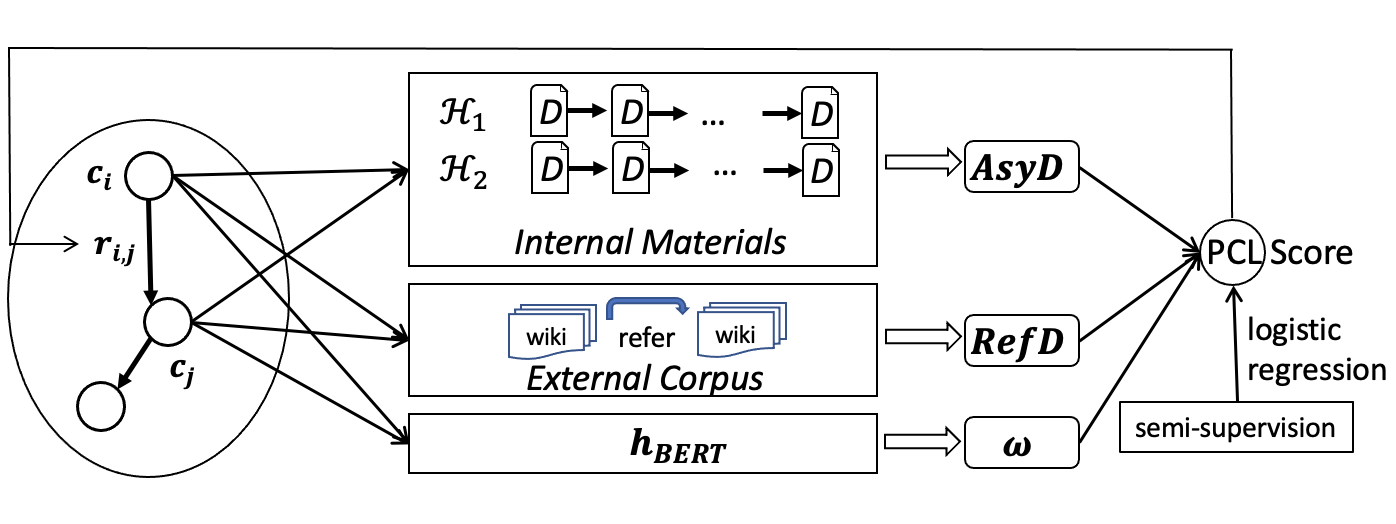
\includegraphics[width=0.50\linewidth]{res/framework_sub1.png}}
% 	\quad 
	\subfigure[Prerequisite Context Modeling in Recommendation]{
		\label{level.sub.2}
		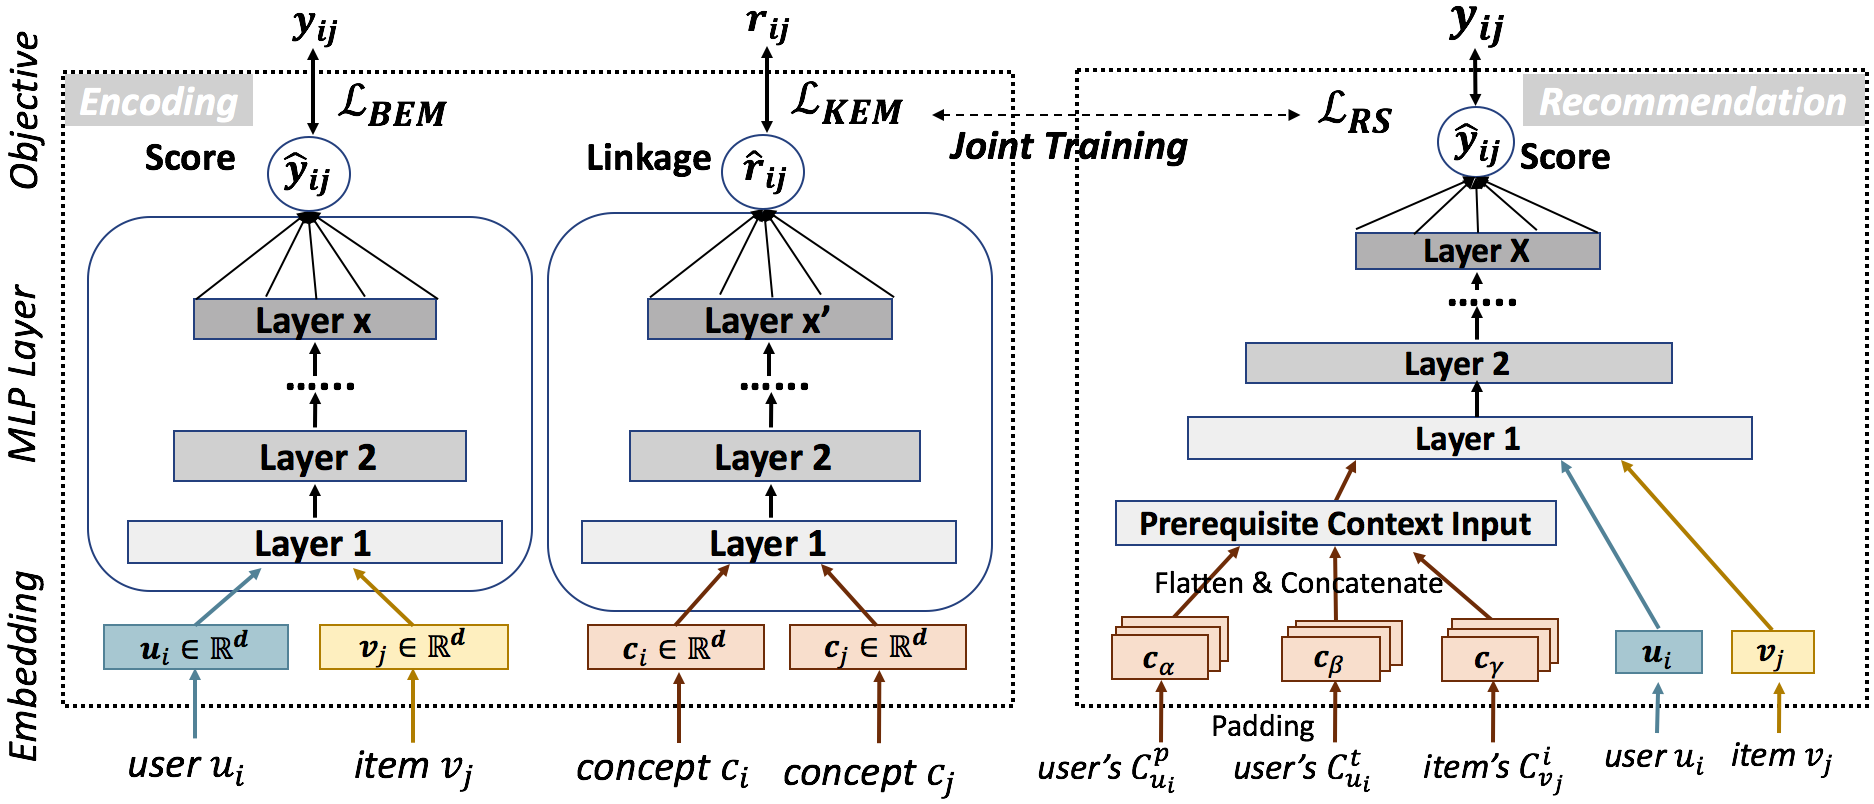
\includegraphics[width=0.48\linewidth]{res/subframwork.png}}
	\caption{Our instantiated neural PDRS framework. It consists components of a) prerequisite constructor,  b [left]) twin encoders pretrain embedding of users, items (BEM), and prerequisites (KEM), and b [right]) a fine-tuned neural recommendation system.}
	\label{fig:framework}
\end{figure}

\section{PDRS: Prerequisite-Driven RS}
%We present a simple yet effective instantiation of PDR, which guides the recommendation task with the encoded prerequisite context.
%To imbue recommendation to capture prerequisites knowledge in a PDR task, 
Our instantiated framework (PDRS) is depicted in Figure~\ref{fig:framework}.  It consists of three components (\S 3.1, 3.2~and~3.3):

% % Min: this doesn't belong here.  It belongs in the dataset part.  It is not a component of your framework.
% \subsection{Prerequisite Context Modeling}

% To the best of our knowledge, no existing dataset is specifically designed for \textit{prerequisite context} modeling.  
% % Min: make these a hyperref URLs
% Hence, we modify existing datasets SSG-Data, MovieLens, and Amazon Books\footnote{(S) https://www.skillsfuture.gov.sg/, (M) https://grouplens.org/datasets/movielens/, and (A) https://jmcauley.ucsd.edu/data/amazon/ \label{fn:web}}
% % to study the role of prerequisites in recommendation.
% % Min: we don't know what ``item documents'' are.
% which all contain textual descriptions of items, which we deem as item documents.
% % In order to thoroughly investigate the potential of this special type of context, 
% % the dataset should include the user's state of knowledge and a rich knowledge concept graph bridging user and item.
% For obtaining user's state of knowledge $\mathcal{K}_u^p$, $\mathcal{K}_u^t$, 
% we assume that users have mastered the knowledge contained in items that they have previously interacted with,
% and take concepts from the
% % Min: items? documents?
% documents of first 30\% and the last 20\% of items they interacted with as their prior and target knowledge, respectively.
% To maintain strict training and testing separation, we only use the remaining 50\% of knowledge concepts for training and testing our PDRS. 
% We also follow the common practice \cite{lei2020interactive} and only retain user records with more than three interactions, to ensure each user has at least one item for evaluating recommendation performance and one item each for modeling prior and target knowledge.

\subsection{Prerequisite Knowledge Inference}
To leverage prerequisite context, we first need to build a \textit{prerequisite graph} with concept-level prerequisite links.
We decompose this process into two subtasks: 
extracting concepts from item descriptions, 
and inferring prerequisite relation between concepts from the ordered item documents and general knowledge (topological relations in Wikipedia).


% \vspace{0.12cm}
% \noindent 
\textbf{Concept Extraction.}
\label{sec:data_construct}
% Our concept extraction procedure identifies and links concepts into a graphical network.  
To extract key concepts from item documents (item description title, and item description content) as prerequisite context,
we extend prior work \cite{pan2017course} on graph propagation as a three-step subprocess.
First, \textit{seed concepts} are extracted from item $v$'s document titles using TextRank \cite{mihalcea2004textrank} (with an empirically tuned threshold of 50\%).
% Min: this clause is more confusing than helpful.  Omit.
% which indicate $v$'s central topics. 
Next, \textit{candidate concepts} are gathered from $v$'s document content, identifying all phrases that match the part-of-speech tag pattern for a noun phrase: $((A|N)+|(A|N)^{*}(NP)?(A|N)^{*})N$ \cite{justeson1995technical} (here, $A$, $N$, and $P$ indicate adjectives, nouns, and prepositions). 
% Min: what is seed-candidate? seed-relevant? Confusing.  I don't know what these qualifiers mean.  These lines 46--49 need re-writing and careful editing that doesn't introduce more difficulties. 
% Holden: added description for clarification below.
Lastly, we construct a fully-connected graph to include both seed concepts and candidate concepts, and expand the seed concept set to cover its relevant concepts. We implement this by iterative propagation, where concepts' confidence scores
(where seed concepts are initially weighted with unit confidence)
are propagated to their neighbors\footnote{For computational efficiency, we only propagate when edge scores are above a tunable parameter $\lambda$.} regarding their semantic relatedness, as measured by cosine similarity $\omega(c_{i},c_{j})=cosine(h_{BERT}(c_{i}),h_{BERT}(c_{j}))$ of the textual meaning $h$ from BERT \cite{devlin2018bert}. 

% \vspace{0.12cm}
% \noindent 
\textbf{Inferring Prerequisites.} Knowledge concepts are then associated by prerequisite relations. 
As shown in Fig~\ref{fig:framework}(a), we obtain the final linking scores by considering three features: 
i) asymmetric sequential interaction distance, 
ii) reference distance from general domain,
and iii) semantic relatedness (as defined above).
We explain the former two features:


% \vspace{1.2mm}
\textit{(i) Asymmetric Sequential Interaction Distance.}
We observe that concepts covered in subsequently-consumed
items are often dependent on those in previous ones; i.e., they are prerequisites. 
% Min: BUG choose a concept in your Fig. 1.  Max Likelihood is no longer there. Holden: Fixed
For example, courses that relate to \textit{Bayes' Theorem} are more likely to appear in a user's interaction history \textit{before} those related to \textit{Hidden Markov Model}.
We introduce Asymmetric Sequential Interaction Distance (AsyD) to model this, which captures the distributional pattern of knowledge concept pairs.
Let's say $P(c_i,c_j) = \sum_{u} \sum_{(v_{p}, v_{l}) \in \mathcal{P}_u} tf(c_i, v_{p}) tf(c_j, v_{l})$ indicates the probability of $c_i$ preceding $c_j$ in interaction histories, where $\mathcal{P}_u = \{(v_a,v_b) | v_a, v_b \in \mathcal{H}_u; ts_u(v_a)<ts_u(v_b)\}$ indicates item pairs ordered by timestamp $ts$ in user historical interaction sequence $\mathcal{H}_u$ and $tf(c,v)$ denotes the term frequency of $c$ in item $v$'s documents (e.g., title and description). 
Specifically, if $c_i$ is a prerequisite of $c_j$, the probability $P(c_i,c_j)$ should be greater than the 
% Min: converse.  Please make sure you know these three terms https://www.varsitytutors.com/hotmath/hotmath_help/topics/converse-inverse-contrapositive
converse association $P(c_j,c_i)$.
Thus, our defined Asymmetric Sequential Interaction Distance is a normalized probability: 
$AsyD\left(c_i, c_j\right) = \sigma \{P(c_i,c_j) / P(c_j,c_i) -1\}$.
% \begin{small}
% \begin{equation}
% \setlength{\abovedisplayskip}{1pt}
% \setlength{\belowdisplayskip}{1pt}
%     AsyD\left(k_i, k_j\right) = \sigma \left(\frac{\sum_{u \in \mathcal{U}} \sum_{\left(v_{p}, v_{l}\right) \in \mathcal{P}_u} tf\left(k_i, v_{p}\right) tf\left(k_j, v_{l}\right)}{\sum_{u \in \mathcal{U}} \sum_{\left(v_{p}, v_{t}\right) \in \mathcal{P}_u} tf\left(k_j, v_{p}\right) tf\left(k_i, v_{l}\right)} -1 \right)
% \end{equation}
% \end{small}
% \noindent where $\mathcal{P}_u = \{(v_a,v_b) | v_a, v_b \in \mathcal{H}_u; ts_u(v_a)<ts_u(v_b)\}$ indicates sequential item pairs in user history and $tf(k,v)$ denotes the term frequency of $k$ in item $v$. 
% ($\mathcal{H}_u \subseteq \mathcal{V}$ here represents $u$'s historical interaction sequence.)
% $AsyD\left(k_i, k_j\right)$ is a normalized probability of $k_i$ preceding $k_j$ in interaction histories, where each occurence event is weighted by the concept's frequency in the item's documents (e.g., title and description).  
When $c_i$ and $c_j$ have arbitrary consumption order --- \textit{i.e.}, when they are independent of each other's distribution --- then $AsyD$ = $0.5$. 

% \vspace{0.1cm}

%% Min: original version commented out.
% \textit{(ii) Wikipedia Reference Distance.}
% Contextual knowledge from general information sources, such as Wikipedia, can also be useful in identifying prerequisite relations.  
% We propose a domain-adaptive Reference Distance ($RefD$) which builds on Liang's work \cite{liang2015measuring} on Wikipedia. 
% As concepts may not be present in Wikipedia,
% we deduce prerequisite relations between concepts $c$ (in our domain) by calculating the normalized distance scores from related Wikipedia concepts $t$ (general domain).
% yiding: how do you identify their related Wikipedia concepts? Holden: add words to explain it. Holden: I don't want to add words to introduce more confuse. it is explained later below.
% The relatedness between $k$ and $t$ is measured by semantic similarity $\omega$.
% For a concept $k$, we consider its related concepts in Wikipedia as $t$, where the similarity is measured by the aforementioned semantic relatedness $\omega(t,k)$: 
% Our $RefD(c_i, c_j)$ measures the imbalance between each pair of $c_i$ and $c_j$ from the reference imbalance $\tau(t_i, t_j)$ in Wikipedia.
% The reference imbalance $\tau=1$ if and only if $t_{i}$ refers to $t_{j}$ in any Wikipedia article but where $t_{j}$ never refers to $t_{i}$. $\tau=-1$ in the converse scenario, and $\tau=0$ if $t_{i}$ and $t_{j}$ co-refer to each other.
% Formally, $RefD(c_i, c_j)=\mathcal{N} \cdot \sum_{i,j} \tau(t_i,t_j) \cdot S_{i,j}$, where $S_{i,j}= \omega(t_i,c_i) \omega(t_j,c_j)$ is used to represent how closely $c_i$ and $c_j$ are linked to their related Wiki concepts, and $\mathcal{N}=(\sum_{i,j} S_{i,j})^{-1}$ is the normalization term.
% $RefD(c_i, c_j)=\sum_{i,j} \tau(t_i,t_j) \cdot S_{i,j}/\sum_{i,j} S_{i,j}$, where the denominator is for normalization.
% This process transforms the concept linking task to one of locating related concepts in Wikipedia. 

\textit{(ii) Wikipedia Reference Distance.}
Textual evidence of prerequisites in domain documents can be sparse, resulting in noisy learned prerequisites.  
Contextual knowledge from general information sources, such as Wikipedia, can aid the identification of prerequisite relations by providing supplemental evidence.  
We observe that related general information that refer to domain concepts can also provide statistical evidence of prerequisites. 
To capture this, we propose a domain-adaptive Reference Distance ($RefD$) which builds on Liang's work \cite{liang2015measuring} on Wikipedia. 
% MinCR => Hengchang: can you give a hypothetical example of $t$ related to $c$ in Fig 1?
%% >> 
For example, the in-domain concept $c$ -- \textit{"probability classifier"} may not occur in Wikipedia, we measure its reference imbalance through its related concepts $t$ -- \textit{"bayes classifier"} in Wiki corpus.
Specifically, when a related concept $t$ is present in Wikipedia that refers to concept $c$, we capture its reference ratio, similar to $AsyD$, by calculating its normalized distance score.
% yiding: how do you identify their related Wikipedia concepts? Holden: add words to explain it. Holden: I don't want to add words to introduce more confuse. it is explained later below.
% The relatedness between $k$ and $t$ is measured by semantic similarity $\omega$.
% For a concept $k$, we consider its related concepts in Wikipedia as $t$, where the similarity is measured by the aforementioned semantic relatedness $\omega(t,k)$: 
$RefD(c_i, c_j)$ measures the imbalance between each pair of in-domain concepts $c_i$ and $c_j$ via its associated reference imbalance $\tau$ to general concepts $t$. This process transforms the concept linking task to one of locating related concepts in Wikipedia. 
The reference imbalance $\tau=1$ if and only if $t_{i}$ refers to $t_{j}$ in any Wikipedia article but where $t_{j}$ never refers to $t_{i}$. As such, $\tau$ analogously ranges $[-1,+1]$. Thus, $RefD$ can smoothly incorporate information from general sources ($\tau$), as well as in-domain sources (represented by $AsyD$); i.e., 
% Formally, $RefD(c_i, c_j)=\mathcal{N} \cdot \sum_{i,j} \tau(t_i,t_j) \cdot S_{i,j}$, where $S_{i,j}= \omega(t_i,c_i) \omega(t_j,c_j)$ is used to represent how closely $c_i$ and $c_j$ are linked to their related Wiki concepts, and $\mathcal{N}=(\sum_{i,j} S_{i,j})^{-1}$ is the normalization term.
$RefD(c_i, c_j)=\sum_{i,j} \tau(t_i,t_j) \cdot S_{i,j}/\sum_{i,j} S_{i,j}$, where 
$S_{i,j}= \omega(t_i,c_i) \omega(t_j,c_j)$ is used to represent how closely $c_i$ and $c_j$ are linked to their related Wiki concepts, and the denominator allows $RefD$ to also be interpreted as a normalized probability. 
% MinCR: why in parens?  Demote to footnote?
% HC: removed the parens, and re-contruct the sentence
% $S_{i,j}= \omega(t_i,c_i) \omega(t_j,c_j)$ is used to represent how closely $c_i$ and $c_j$ are linked to their related Wiki concepts.

% $RefD(k_i, k_j)$ indicates the imbalance between $k_i$ and $k_j$ by measuring the reference imbalance between $t_p$ and $t_l$.
%% yiding: what does 'reference imbalance' mean?
%% Min: Agree with Yiding.  This is not clear.  Math is hurting the understanding of what you are doing.  This section also needs careful re-editing.  I don't understand.
% Holden: re-edited
% Formally, $RefD(k_i, k_j)= \{\sum_{t_p,t_l} [\tau(t_p,t_l)-\tau(t_p,t_l)] S_{p,l}(k_i,k_j)\} \cdot \{\sum_{t_p,t_l}S_{p,l}(k_i,k_j)\}^{-1}$, where the reference indicator $\tau(t_p,t_l)$ is equal to 1 if $t_{p}$ refers to $t_{l}$ in an article, and 0 otherwise.
% $S_{p,l}(k_i,k_j) = \omega(t_p,k_i) \cdot \omega(t_l,k_j)$ .
% Thus the second part can be termed as the normalization.


% \vspace{0.12cm}
\textit{Prerequisite Learning.}
To obtain the final prerequisite knowledge linkage scores $PKL(c_i,c_j)$, we train logistic regression over seed annotated samples ($n = 300$ per dataset), as shown on the right part of Fig.~\ref{fig:framework}a. The regression is learned by adjusting the contribution weights for the three features $\omega, AsyD and RefD$ on manually-labeled concept pairs.  We then run the regression to yield output for all knowledge concept pairs. This process reduces noise from the parameters, providing more accurate PKL scores for downstream recommendation (Fig.~\ref{fig:framework}b).
% Our constructed prerequisite data are available at https://github.com/HoldenHu/PDRS/.

\subsection{User/item and Prerequisite Context Encoding}
\label{sec:module2}

The Encoding modules take the sparse input representations of users, items and concepts identified by PKL and encode them into dense representations
% for better performing similarity distances \cite{mikolov2013efficient}.
% yiding: what's 'better performing similarity distances'? easy computation of similarity measures?
(Fig.~\ref{fig:framework}b [left]), employing a multi-layer perceptron (MLP) for both \textit{Knowledge Encoding Module (KEM)} and \textit{Behavior Encoding Module (BEM)}.

% Holden: @Min to recheck this expression below.
% yiding: the following paragraph is a bit confusing 
KEM learns the knowledge concept embedding by training pairs of $(c_i,c_j)$ to approximate their previously-assigned prerequisite PKL scores. 
% Min: how does the math help here?  It is confusing
% Formally, it optimizes the parameters $\operatorname{argmin}_{\Phi} \sum_{(i,j)} \mathcal{L}_{KEM}(r_{i,j}, \hat{r}_{i,j})$, where $r_{i,j}$ is expected prerequisite weight $PKL(k_i,k_j)$, and $\hat{r}_{i,j}$ is the estimated output from a $x$-layer $MLP_{x}({k_i}, {k_j}, \Phi)$ which interacts the factors from concatenated embedding of $k_i$ and $k_j$.
Our target in this step is to obtain every concept $c$'s embedding $\mathbf{c} \in \mathbf{\mathbb{R}^{1 \times d}}$ by tuning the learnable parameters $\Phi$
to achieve the minimized $\mathcal{L}_{KEM}(r_{i,j}, \hat{r}_{i,j})$, where $r_{i,j}$ is expected prerequisite weight $PKL(k_i,k_j)$, and $\hat{r}_{i,j}$ is the estimated output from a 
% MinCR: I don't think the x notation helps to make anything more clear.  Dropping.  Please check.
% $x$-layer MLP.
MLP.
% \vspace{-0.1cm}
BEM works similarly, learning user/item embeddings by minimizing the difference $\mathcal{L}_{BEM}$ between predicted 
% MinCR: why x'?  Obsolete anyways.
% $\hat{y}_{i,j} = MLP_{x'}(u_i, v_j, \Theta)$ 
$\hat{y}_{i,j} = MLP(u_i, v_j, \Theta)$ 
and the truth $y_{i,j}$. 
% Min: again the math doesn't help (to me). 
% Formally, it targets at learning $\operatorname{argmin}_{\Theta} \sum_{(i,j)} \mathcal{L}_{BEM}(y_{i,j}, \hat{y}_{i,j})$ projecting $u_i$, $v_j$ to their embedding $\mathbf{u}_i$, $\mathbf{v}_j$ separately.
We select a mean-squared loss for $\mathcal{L}_{KEM}$
% $ = \sum_{i,j}(\hat{r}_{i,j}-r_{i,j})^{2}$  
to best model the real-valued prerequisite scores, and a binary cross entropy loss for $\mathcal{L}_{BEM}$.
%$ = -\sum_{i,j} (y_{i,j} \times ln (\hat{y}_{i,j}) +(1-y_{i,j} \times ln(1-\hat{y}_{i,j})))$.

%%%%%%%%%%%%%%%%%%%%%%%%%%%%%%%%%%%%%%%%%%%%%%%%%%%
% Module 3
%%%%%%%%%%%%%%%%%%%%%%%%%%%%%%%%%%%%%%%%%%%%%%%%%%%
\subsection{Recommendation Module}
\label{sec:module3}
As shown in Fig.~\ref{fig:framework}b [right],
PDRS combines the embedded representation of user context (user prior knowledge concepts $C^p_u$ and target knowledge concepts $C^t_u$) and item context (item concepts $C_v^i$) to output the final recommendation prediction $\hat{y}_{ij}$. We apply the average pooling for the concept embedding, while a user/item corresponds to multiple knowledge concepts. Formally, $\hat{y}_{uv}=MLP\{\mathbf{u}, \mathbf{v}, avg(\mathbf{C}^p_u), avg(\mathbf{C}^t_u), avg(\mathbf{C}_v^i)\}$,
% user context (user's prior and target knowledge), and item context (item contained knowledge)
% We minimise difference between ground truth and prediction, using the embedded representation of the input: 3-tuples consisting of a concatenation of the average embedding of 1) user prior knowledge $K^p_u$, 2) target knowledge $K^p_t$, 3) item knowledge $K$.
% \vspace{-0.1cm}
% \paragraph{Pre-training.} 
where BEM and KEM provide the pre-trained embeddings $\mathbf{u}$, $\mathbf{v}$, and $\mathbf{c}$ for the user, item and prerequisite contexts, respectively.
% Outputs from the encoding process (KEM and BEM) initialize encoding layers $\mathbf{K}, \mathbf{V}, \mathbf{U}$ to map $k,v,u$ to their corresponding embeddings $\mathbf{k},\mathbf{v},\mathbf{u}$, as a form of pre-training.  
We further tune the embedding parameters through joint training that alternately applies the objective of $\mathcal{L}_{KEM}$ and the final recommendation $\mathcal{L}_{Rec}$.  $\mathcal{L}_{Rec}$ is also a binary cross entropy loss between model prediction $\hat{y}$ and the ground truth interaction $y$.
% When training the recommendation module, $\mathbf{K}, \mathbf{V}, \mathbf{U}$ are then fine-tuned.

% \vspace{-0.1cm}
% \paragraph{Joint Training}
% The training of the recommendation module optimizes $\mathbf{K,V,U}$ for only the recommendation task. As a side effect, this optimisation weakens the prerequisite information stored in $\mathbf{K}$, gradually learning collaborative patterns. For example, if users tend to study \textit{Python} and \textit{Photoshop} together, their learned representations will be similar in $\mathbf{K}$.

% We design PDRS to benefit primarily from the pre-trained prerequisite information.  As such. we expect the pre-trained $\mathbf{K}$ should not change much.  Freezing such pre-trained weights is possible, but shown to be suboptimal \cite{kwok1993experimental}.
% Experimental analysis of input weight freezing in constructive neural networks
%% Min5: consider showing how much this alternating training actually helps performance.  Is it an important detail? 
% We solve this by alternately training for two objectives: a mean-squared loss for prerequisite representation ($\mathcal{L}_{KLP}$; in the Encoder) and a binary cross entropy loss for final recommendation ($\mathcal{L}_{RS}$; in the Recommender):

% \vspace{-0.3cm}
% \begin{eqnarray}
% \setlength{\abovedisplayskip}{-0.1pt}
% \setlength{\belowdisplayskip}{0pt}
%     \mathcal{L}_{KLP}= &\sum_{i,j}(\hat{r}_{i,j}-r_{i,j})^{2} \\
%     \mathcal{L}_{RS}= & -\sum_{i,j} (y_{i,j} \times ln (\hat{y}_{i,j}) +(1-y_{i,j} \times ln(1-\hat{y}_{i,j}))) 
% \end{eqnarray}

We empirically observe that the joint training of losses $\mathcal{L}_{KEM}$ and $\mathcal{L}_{Rec}$ enables the model to focus on prerequisite information.  It also reduces the time complexity to a linear $O(|Y|+|R|)$ from the total quadratic complexity $O(\frac{|Y| \times |R| \times (dY+dR)}{dY \times dR})$ of alternatively executing the two objectives (where $dY$ and $dR$ represent the batch sizes of interaction and prerequisite pairs, respectively).
